% !TEX root = ../thesis-example.tex
%
\chapter{System Design and Implementation}
\label{sec:system}

\section{Work Setting}
We use an Intel Realsense camera model D435I as can be seen in \href{https://www.intel.com/content/www/us/en/products/sku/190004/intel-realsense-depth-camera-d435i/specifications.html}{Intel's official specification}. Its technical specs are the following:
\begin{itemize}
	\item Resolution:1280x720
	\item Depth Field of View: 87 degrees wide horizontally, 58 degrees vertically
	\item FPS:30
	\item Operating range: Min. 0.3m, Max 3m
\end{itemize}
The setting is at an office, an indoor place, with either not harsh natural light or
normal overhead office lights.
What we want to achieve is to cover people and faces that appear in the point cloud
frame of the camera using a simple blurring effect. There are more advanced techniques
for anonymization as previously discussed, such as the sophisticated face swapping demonstrated in \cite{Zhao_Zhang_Demiris_2024}.

\section{Demonstration}
\label{sec:system:sec0}
The software works by first reading the depth and color frame at each iteration of the program.
Then, different face or people detection modules run using the depth and color frames as data
returning a label and a box in either 2D or 3D coordinates based on the data it is operating on.
2D object detection modules can use only the color frame to run their detection.
Finally the rendering engine applies all the blurring effects based on the detection results and renders
the resulting pointcloud as it can be seen in \ref{fig:system:2}.
A trivial semantic segmentation scenario was implemented using the RANDLaNet and KPFCNN models
provided with pretrained weights from a library we used. The results looks like the figure \ref{fig:system:4}.
An unsuccessfull 3D object detection was attempted using the PointPillars model from \cite{Lang_Vora_Caesar_Zhou_Yang_Beijbom_2019}. The failure most likely stems from improper configuration for our scenario and the specific camera specifications.

\begin{figure}[htb]
	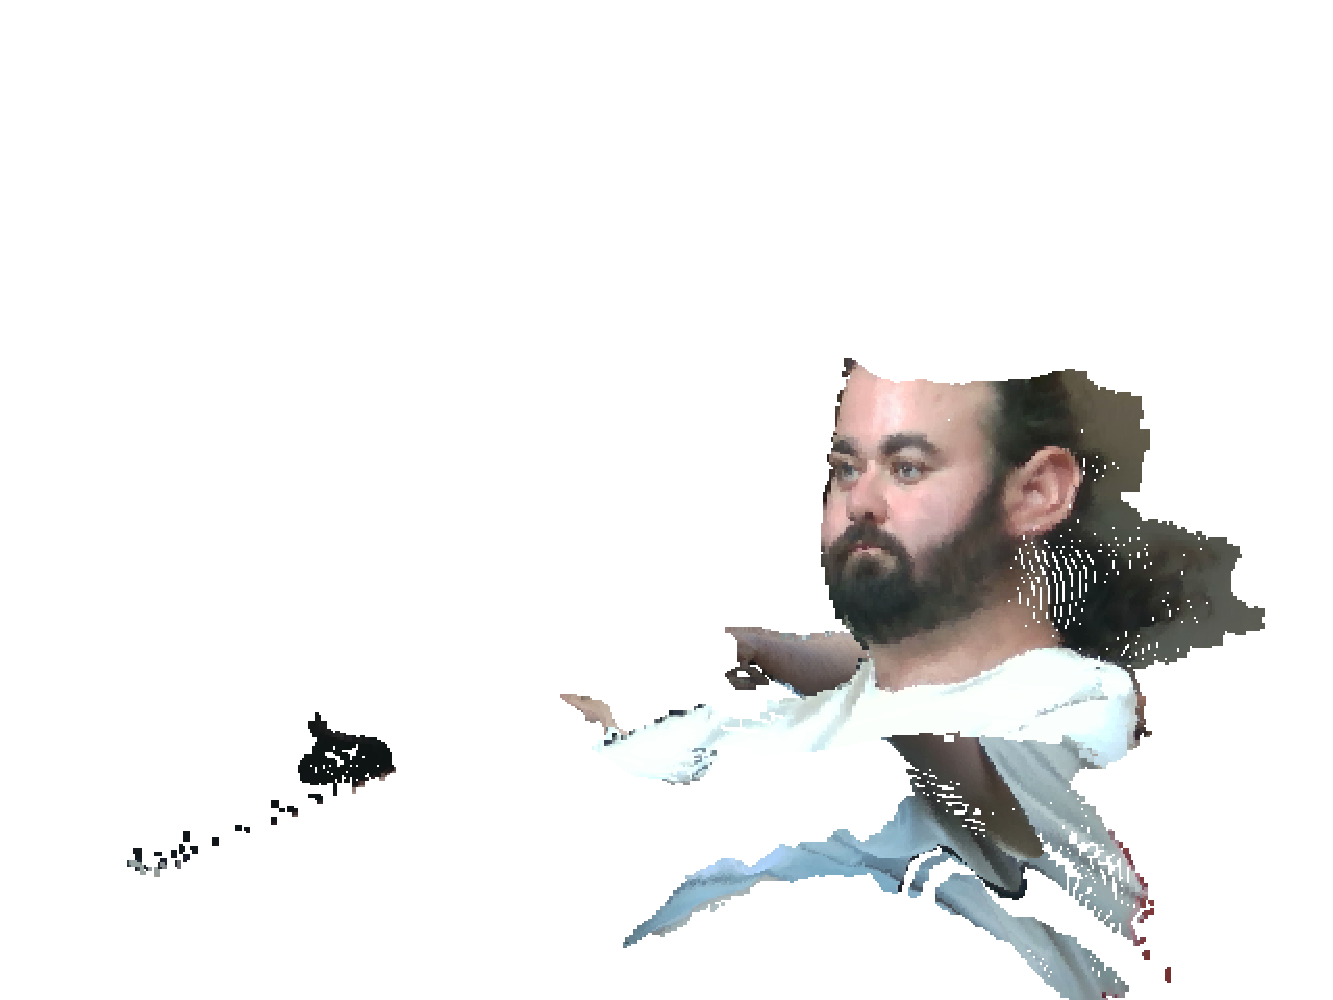
\includegraphics[width=\textwidth]{figs/Pointcloud-Face-Without-Blur.pdf}
	\caption{Point cloud rendered without blurring faces and people}
	\label{fig:system:1}
\end{figure}

\begin{figure}[htb]
	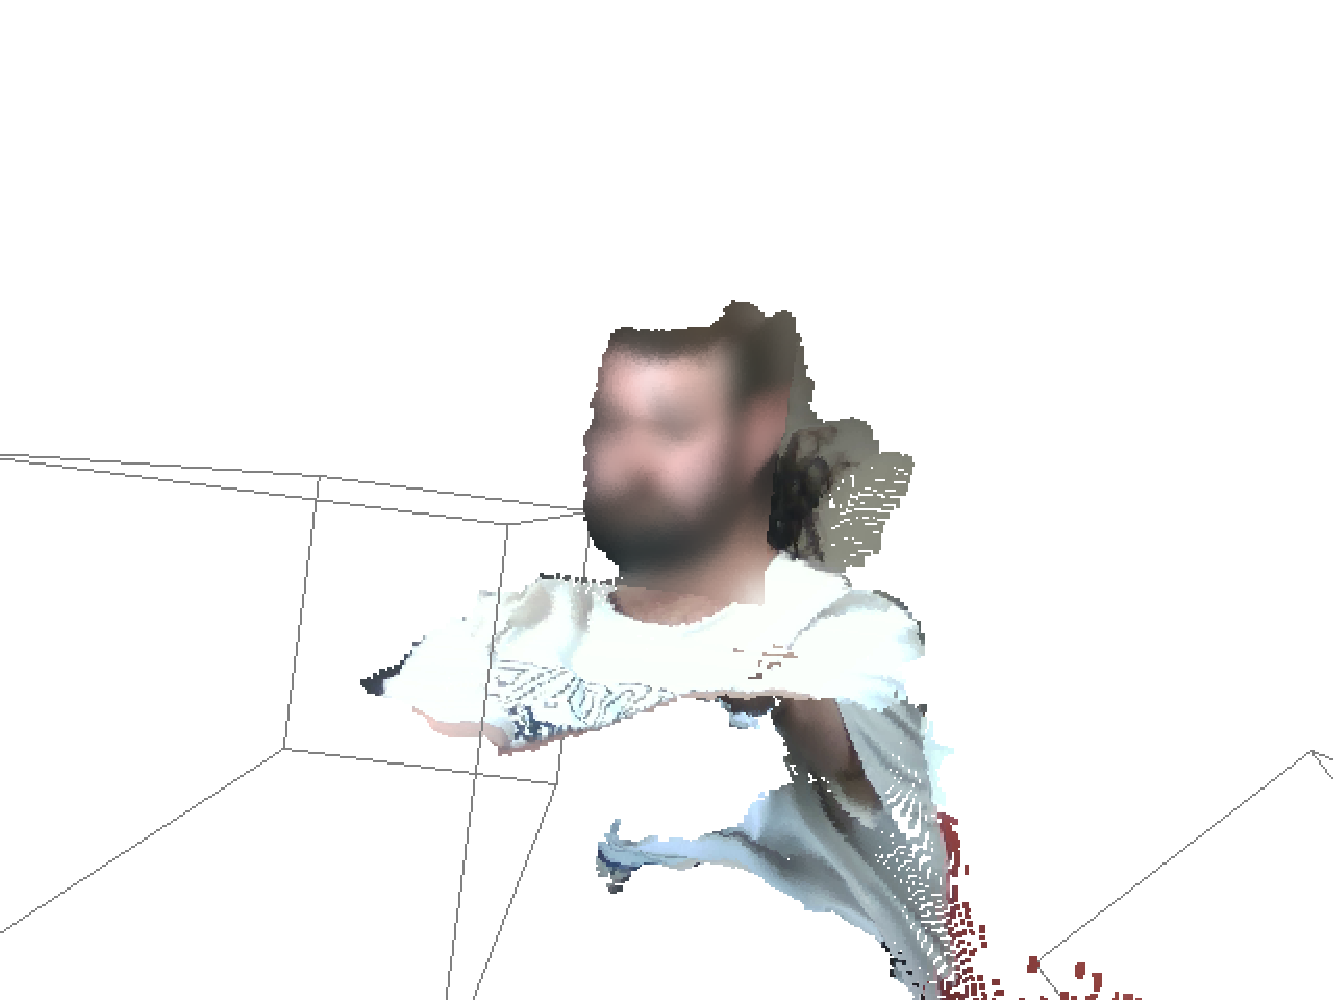
\includegraphics[width=\textwidth]{figs/Face-Blurred-With-2D-Detection-And-Blur.pdf}
	\caption{Point cloud rendered with blurred faces(The bounding box demonstrates we can also add 3D detections)}
	\label{fig:system:2}
\end{figure}

\begin{figure}[htb]
	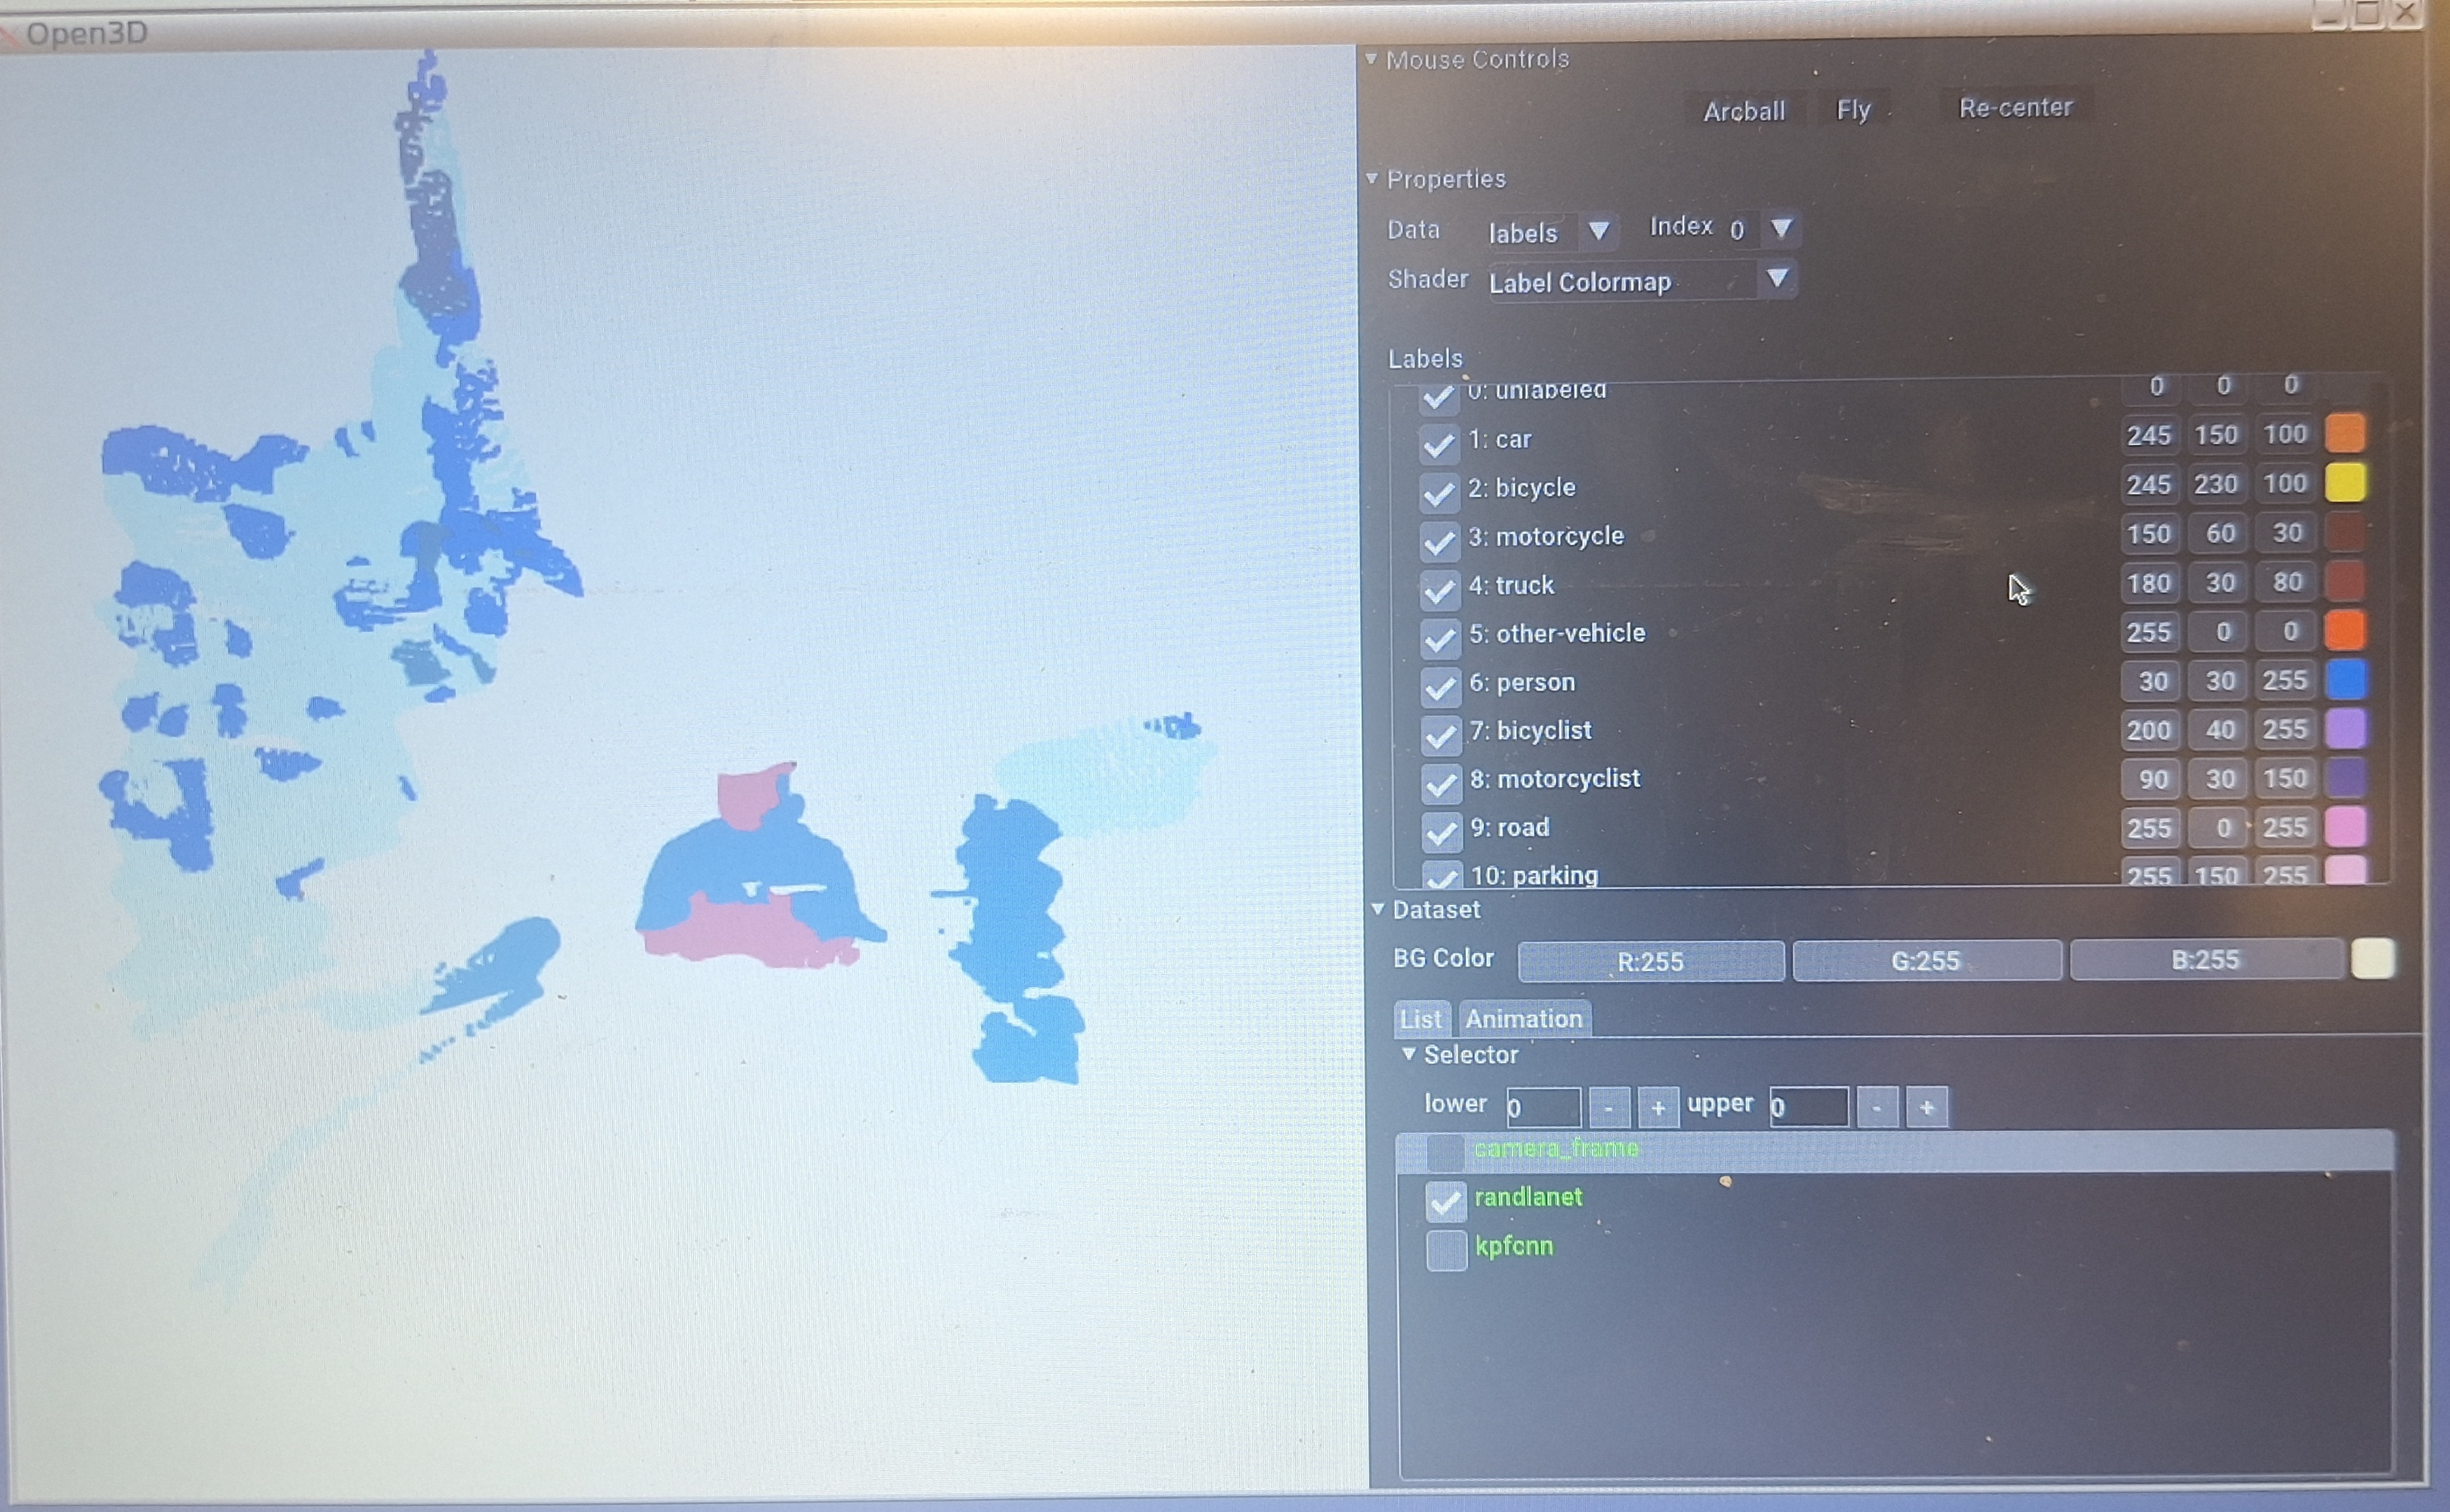
\includegraphics[width=\textwidth]{figs/Semantic-Segmentation-Example.pdf}
	\caption{Semantic segmentation using RandLaNet and KPFCNN from Open3D library.}
	\label{fig:system:4}
\end{figure}

\section{Design}
\label{sec:system:sec1}
The design of this system is not too sophisticated as this is a proof of concept prototype.
Nonetheless some work has been done on the architecture to ensure features can be added seamlessly
as it can be seen in \ref{fig:system:3}.
A CameraReader interface was made in order to be able to support cameras from different manufacturers,
and possibly a camera that its frames are streamed over the network.
The EffectsManager class is responsible for all of the tools that will operate on the depth, color and
point cloud data. It ensures that all of the detection tools use as input the same data without mutations.
In addition, it could allow for running the detections in parallel for better performance and for toggling
tools on and off based on certain conditions or user input.

\begin{figure}
	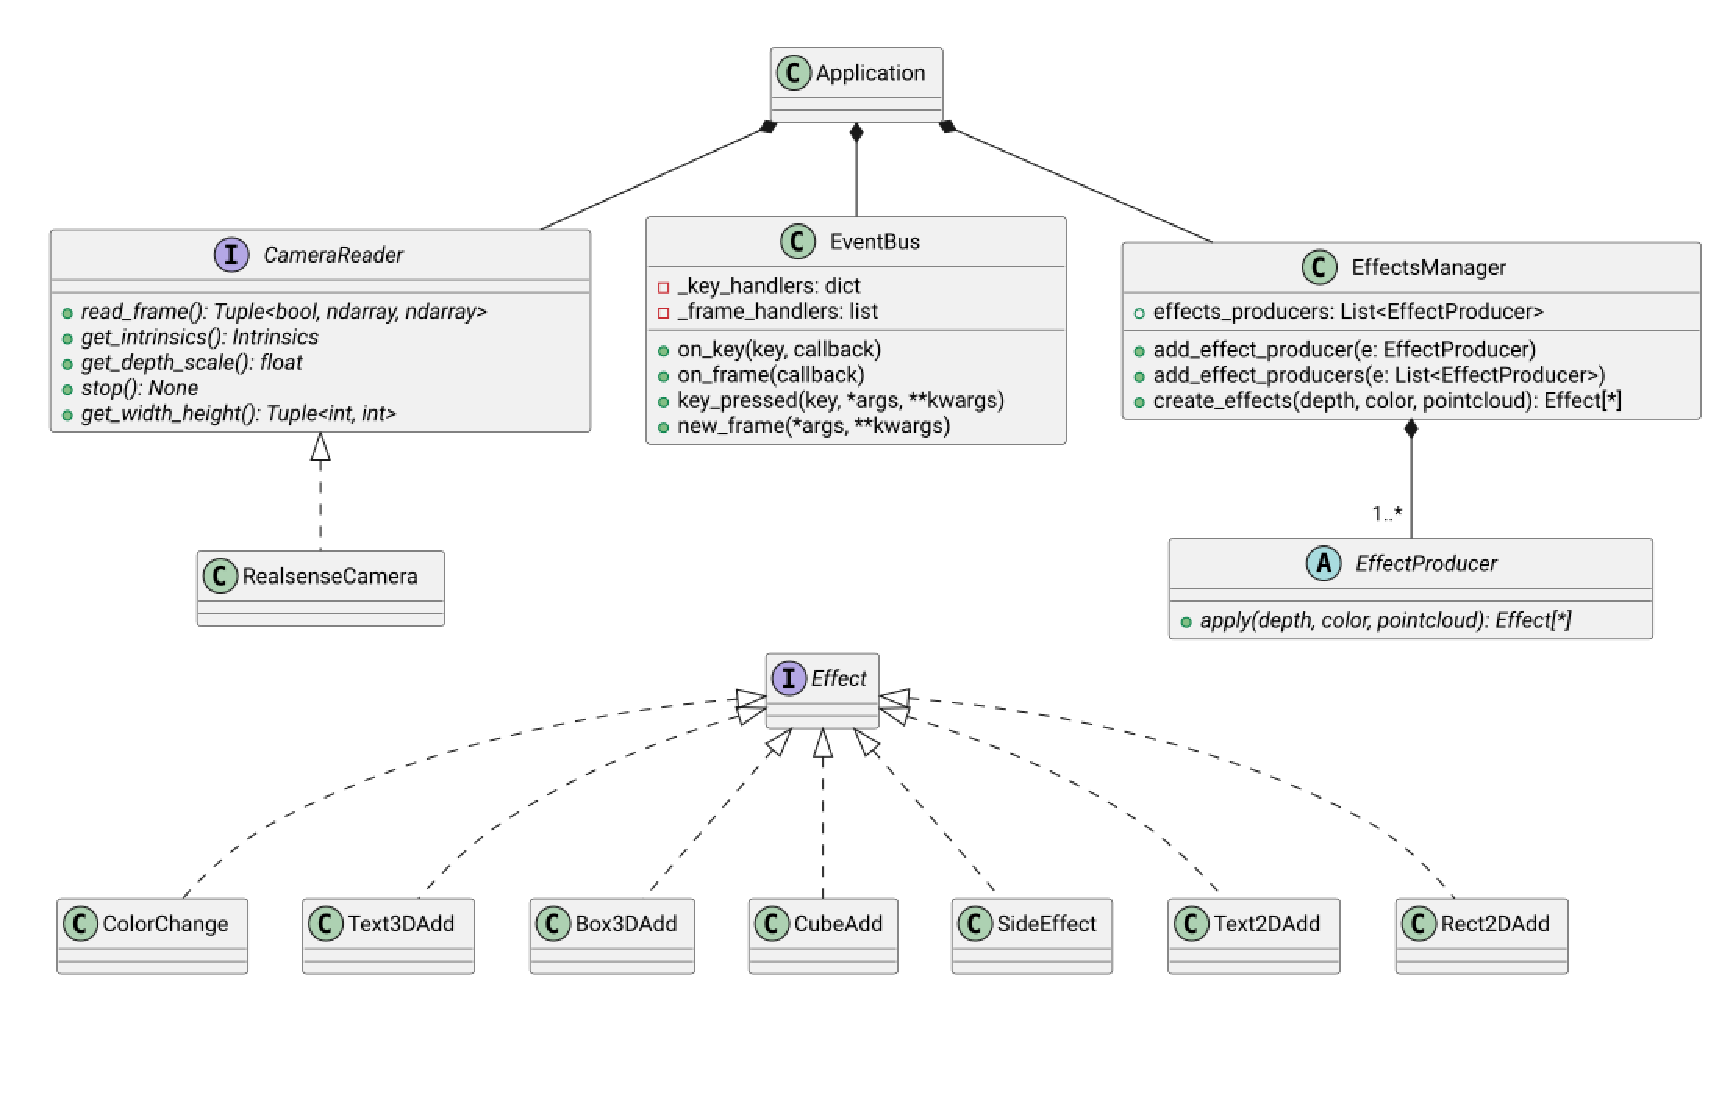
\includegraphics[width=\textwidth]{figs/Uml-Diagram-Thesis-Final.pdf}
	\caption{UML Class Diagram for system architecture}
	\label{fig:system:3}
\end{figure}

\section{Implementation}
\label{sec:system:sec2}
Python was the programming language of choice in this project, as most AI related models and libraries
support python. Another reason was to speed up development, otherwise it would make more
sense to implement everything in C++ as AI models and related libraries are usually implemented in it.
Several tools were used in order to focus more on the use case and less on the implementation
details outlined in \ref{fig:technologies}.
\href{https://github.com/isl-org/Open3D}{\emph{Open3D}} is a C++ based library with a python wrapper for convenience made by the Intelligent Systems Lab organization from Intel for processing and visualizing \ac{PC}s.
\href{https://github.com/isl-org/Open3D-ML/}{\emph{Open3D-ML}} is an extension to the open3D library that focuses on AI-based tasks such as object detection and semantic segmentation.
It supports both PyTorch and Tensorflow as the 3D machine learning base tool and supports GPU acceleration for computationally expensive 3D operations.
Both libraries are properly maintained and were used in this work.
For 3D object detection only the PointPillars and PointRCNN models are implemented and pretrained on the KITTI dataset in both PyTorch and Tensorflow implementations.

\href{https://opencv.org/}{\emph{OpenCV}} is the industry standard when it comes to computer vision in 2D scenarios. We used this library for doing 2D face detection as a fallback because the \ac{PC} based models were too complicated to setup and expensive to fine-tune. More specifically we used the Haar Cascade Classifier in openCV that is based on early machine learning work at \cite{Viola_Jones_2001}.
OpenCV was also used to implement blurring in an image as the 3D equivalent would be more computationally expensive.
Gaussian blurring replaces each pixel's value with a weighted average of its neighboring pixels.
Gaussian as the weights follow a Gaussian distribution, which in this case results in pixels closer to the center contributing more than the pixels further away to the final color of the blurred pixel.


We also used the OpenCV DNN module to do general object detection using a MobileNet-SSD implementation with pretrained weights and network architecture provided by a \emph{.caffemodel} and a \emph{.prototxt} file respectively.
We used \href{https://pypi.org/project/pyrealsense2/}{\emph{Pyrealsense2}} from Intel's official SDK for Realsense cameras,for interfacing with the camera D435I.

\begin{figure}[h]
	\centering
	\begin{tikzpicture}[
			box/.style={rectangle, rounded corners, draw, minimum width=2.5cm, minimum height=1.5cm, align=center, font=\small},
			category/.style={rectangle, rounded corners, draw, fill=gray!20, minimum width=3.5cm, minimum height=0.8cm, align=center, font=\small\bfseries}
		]
		% 2D Processing
		\node[category] (2d) at (0, 6) {2D Processing};
		\node[box] (opencv) at (3.5, 6) {%
			
\includegraphics[height=0.6cm]{figs/opencv.png}\\OpenCV};
		\node[box] (haar) at (6.5, 7) {Haar Cascade\\{\tiny Face Detection}};
		\node[box] (dnn) at (6.8, 5) {DNN Module\\{\tiny Object Detection, MobileNet-SSD}};
		\draw[->] (2d) -- (opencv);
		\draw[->] (opencv) -- (haar);
		\draw[->] (opencv) -- (dnn);

		% 3D Processing
		\node[category] (3d) at (0, 3) {Point cloud Processing \\ \& Visualization};
		\node[box] (open3d) at (3.5, 3) {%
			
\includegraphics[height=0.6cm]{figs/open3d.png}\\Open3D};
		\draw[->] (3d) -- (open3d);

		% 3D ML
		\node[category] (3dml) at (0, 1) {3D Object Detection \&\\Segmentation};
		\node[box] (open3dml) at (3.5, 1) {%
		
\includegraphics[height=0.6cm]{figs/open3dml.png}\\Open3D-ML\\{\tiny PointPillars, PointRCNN}};
		\draw[->] (3dml) -- (open3dml);

		% Camera
		\node[category] (cam) at (0, -1) {Camera};
		\node[box] (rs) at (3.5, -1) {Pyrealsense2\\{\tiny Python Wrapper}};
		\node[box] (cam2) at (7.0, -1) {%
			
\includegraphics[height=0.6cm]{figs/realsense.png}\\RealSense D435I};
		\draw[->] (cam) -- (rs);
		\draw[->] (rs.east) -- (cam2.west);

	\end{tikzpicture}
	\caption{Technologies used in the system implementation}
	\label{fig:technologies}
\end{figure}

Tools that were not used that could otherwise be useful are the following:
\begin{itemize}
	\item \href{https://github.com/open-mmlab/OpenPCDet}{\emph{OpenPCDet}}, it heavily depended on CUDA without AMD GPU/CPU equivalents which was not available in this work.
	\item \href{https://github.com/open-mmlab/mmdetection3d}{\emph{MMDetection3D}}, supports lots of models we reviewed but had issues when trying to integrating with our work, a great tool nonetheless. In detail, the problem was that it required a different version of PyTorch(1.8+) in contrast to Open3D (2.2+).
	\item \href{https://github.com/vinits5/learning3d}{\emph{Learning3D}}, does not support many models, we tried to use it and did not have the desired results. Also integrating with our existing code would be infeasible as it required pytorch 1.3+ and a CUDA GPU.
	\item \href{https://github.com/NVIDIA-AI-IOT/CUDA-PointPillars}{\emph{CUDA-PointPillars}}, a CUDA optimized implementation of PointPillars from NVIDIA that achieves comparable detection performance but at considerable less time, 6.84ms.
\end{itemize}
